% Explanatory geometry, not converter data or a nonlinear invariant set.
% Unit sublevel: V(z) = z_1^2/9 + z_2^2/2.25 <= 1.
% The point (1.8, 1.2) is on its boundary. Both endpoint images are
% strictly inside; the marked intermediate image is their midpoint.
% Included by main.tex; compiled directly by task build.
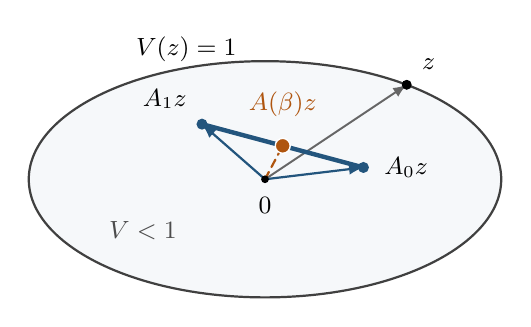
\begin{tikzpicture}[font=\small, >=latex, line cap=round, line join=round]
    \definecolor{certblue}{RGB}{35,85,125}
    \definecolor{certorange}{RGB}{175,85,15}
    \coordinate (O) at (0,0);
    \coordinate (z) at (1.8,1.2);
    \coordinate (a0) at (1.25,0.15);
    \coordinate (a1) at (-0.8,0.7);
    \coordinate (ab) at (0.225,0.425);

    \filldraw[fill=certblue!4, draw=black!75, line width=0.8pt]
        (O) ellipse [x radius=3cm, y radius=1.5cm];
    \node at (-1.0,1.65) {$V(\vect{z})=1$};
    \node[text=black!70] at (-1.55,-0.65) {$V<1$};

    \draw[->, black!60, line width=0.7pt] (O) -- (z);
    \draw[->, certblue, line width=0.8pt] (O) -- (a0);
    \draw[->, certblue, line width=0.8pt] (O) -- (a1);
    \draw[certblue, line width=1.6pt] (a0) -- (a1);
    \draw[densely dashed, certorange, line width=0.8pt] (O) -- (ab);

    \fill (O) circle [radius=1.4pt];
    \fill (z) circle [radius=1.8pt];
    \fill[certblue] (a0) circle [radius=2pt];
    \fill[certblue] (a1) circle [radius=2pt];
    \filldraw[fill=certorange, draw=white, line width=0.5pt]
        (ab) circle [radius=2.7pt];

    \node[below=3pt] at (O) {$\vect{0}$};
    \node[above right=2pt] at (z) {$\vect{z}$};
    \node[right=4pt] at (a0) {$A_0\vect{z}$};
    \node[above left=2pt] at (a1) {$A_1\vect{z}$};
    \node[above=7pt, text=certorange] at (ab) {$A(\beta)\vect{z}$};
\end{tikzpicture}
